% Options for packages loaded elsewhere
\PassOptionsToPackage{unicode}{hyperref}
\PassOptionsToPackage{hyphens}{url}
%
\documentclass[
  ignorenonframetext,
  aspectratio=169]{beamer}
\usepackage{pgfpages}
\setbeamertemplate{caption}[numbered]
\setbeamertemplate{caption label separator}{: }
\setbeamercolor{caption name}{fg=normal text.fg}
\beamertemplatenavigationsymbolsempty
% Prevent slide breaks in the middle of a paragraph
\widowpenalties 1 10000
\raggedbottom
\setbeamertemplate{part page}{
  \centering
  \begin{beamercolorbox}[sep=16pt,center]{part title}
    \usebeamerfont{part title}\insertpart\par
  \end{beamercolorbox}
}
\setbeamertemplate{section page}{
  \centering
  \begin{beamercolorbox}[sep=12pt,center]{part title}
    \usebeamerfont{section title}\insertsection\par
  \end{beamercolorbox}
}
\setbeamertemplate{subsection page}{
  \centering
  \begin{beamercolorbox}[sep=8pt,center]{part title}
    \usebeamerfont{subsection title}\insertsubsection\par
  \end{beamercolorbox}
}
\AtBeginPart{
  \frame{\partpage}
}
\AtBeginSection{
  \ifbibliography
  \else
    \frame{\sectionpage}
  \fi
}
\AtBeginSubsection{
  \frame{\subsectionpage}
}
\usepackage{amsmath,amssymb}
\usepackage{lmodern}
\usepackage{iftex}
\ifPDFTeX
  \usepackage[T1]{fontenc}
  \usepackage[utf8]{inputenc}
  \usepackage{textcomp} % provide euro and other symbols
\else % if luatex or xetex
  \usepackage{unicode-math}
  \defaultfontfeatures{Scale=MatchLowercase}
  \defaultfontfeatures[\rmfamily]{Ligatures=TeX,Scale=1}
\fi
\usetheme[]{Frankfurt}
\usecolortheme{orchid}
% Use upquote if available, for straight quotes in verbatim environments
\IfFileExists{upquote.sty}{\usepackage{upquote}}{}
\IfFileExists{microtype.sty}{% use microtype if available
  \usepackage[]{microtype}
  \UseMicrotypeSet[protrusion]{basicmath} % disable protrusion for tt fonts
}{}
\makeatletter
\@ifundefined{KOMAClassName}{% if non-KOMA class
  \IfFileExists{parskip.sty}{%
    \usepackage{parskip}
  }{% else
    \setlength{\parindent}{0pt}
    \setlength{\parskip}{6pt plus 2pt minus 1pt}}
}{% if KOMA class
  \KOMAoptions{parskip=half}}
\makeatother
\usepackage{xcolor}
\newif\ifbibliography
\setlength{\emergencystretch}{3em} % prevent overfull lines
\providecommand{\tightlist}{%
  \setlength{\itemsep}{0pt}\setlength{\parskip}{0pt}}
\setcounter{secnumdepth}{-\maxdimen} % remove section numbering
\ifLuaTeX
\usepackage[bidi=basic]{babel}
\else
\usepackage[bidi=default]{babel}
\fi
\babelprovide[main,import]{brazilian}
% get rid of language-specific shorthands (see #6817):
\let\LanguageShortHands\languageshorthands
\def\languageshorthands#1{}
\ifLuaTeX
  \usepackage{selnolig}  % disable illegal ligatures
\fi
\IfFileExists{bookmark.sty}{\usepackage{bookmark}}{\usepackage{hyperref}}
\IfFileExists{xurl.sty}{\usepackage{xurl}}{} % add URL line breaks if available
\urlstyle{same} % disable monospaced font for URLs
\hypersetup{
  pdftitle={Spatial distributions of job accessibility, housing rents, and poverty: The case of Nairobi},
  pdfauthor={Shohei Nakamura e Paolo Avner (2021)},
  pdflang={pt-BR},
  hidelinks,
  pdfcreator={LaTeX via pandoc}}

\title{Spatial distributions of job accessibility, housing rents, and
poverty: The case of Nairobi\thanks{Apresentador: Arthur Alvarenga}}
\subtitle{Seminário de Econometria Espacial Aplicada}
\author{Shohei Nakamura e Paolo Avner (2021)}
\date{2023-01-18}
\logo{
\includegraphics{yaml/ufjf.png}}

\begin{document}
\frame{\titlepage}

\hypertarget{introduuxe7uxe3o}{%
\subsection{Introdução}\label{introduuxe7uxe3o}}

\begin{frame}{Motivação}
\protect\hypertarget{motivauxe7uxe3o}{}
\textbf{Acessibilidade}

\begin{itemize}
\tightlist
\item
  Acesso a oportunidades \(\rightarrow\) match no mercado de trabalho
  \(\rightarrow\) economias de aglomeração
\item
  Acessibilidade limitada reduz essas oportunidades
\item
  Mais pobres são mais afetados?

  \begin{itemize}
  \tightlist
  \item
    Aprofunda desigualdades
  \end{itemize}
\end{itemize}

\textbf{Mercado imobiliário}

\begin{itemize}
\tightlist
\item
  Oferta limitada em locais com boa acessibilidade
\item
  \emph{Tradeoff}: morar perto ou morar bem?
\end{itemize}
\end{frame}

\begin{frame}{Problemas de pesquisa}
\protect\hypertarget{problemas-de-pesquisa}{}
\begin{enumerate}
\tightlist
\item
  Explorar padrões de acesso ao emprego
\end{enumerate}

\begin{itemize}
\tightlist
\item
  Construir \textbf{índices} de acessibilidade
\item
  Residência formal/informal, qualificação e renda
\end{itemize}

\begin{enumerate}
\setcounter{enumi}{1}
\tightlist
\item
  Analisar o tradeoff no mercado imobiliário
\end{enumerate}

\begin{itemize}
\tightlist
\item
  Modelo hedônico residencial
\item
  Identificar \textbf{prêmio} de mercado da acessibilidade
\end{itemize}
\end{frame}

\begin{frame}{Objeto de pesquisa}
\protect\hypertarget{objeto-de-pesquisa}{}
\begin{columns}

\column{0.5\textwidth}

\textbf{Nairobi}

\begin{itemize}
  \item{Capital do Quênia}
  \item{População:}
    \begin{itemize}
      \item{5 milhões na Região Metropolitana}
      \item{4,4 na cidade}
      \item{Destes, 1 milhão em moradias informais}
    \end{itemize}
\end{itemize}

\column{0.5\textwidth}
\begin{figure}

{\centering 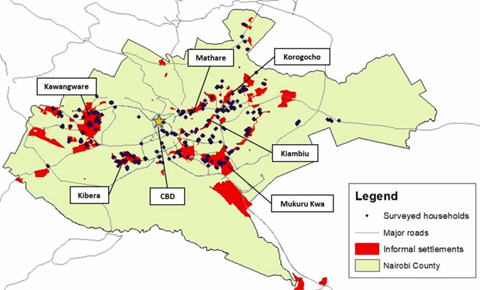
\includegraphics[width=0.7\linewidth]{images/1_survey} 

}

\caption{\label{fig:survey1} Mapa de residências entrevistadas e assentamentos informais. Fonte: Nakamura e Avner (2021)}\label{fig:survey}
\end{figure}
\end{columns}
\end{frame}

\hypertarget{metodologia}{%
\subsection{Metodologia}\label{metodologia}}

\begin{frame}{Acessibilidade}
\protect\hypertarget{acessibilidade}{}
\begin{definition}
Número de oportunidades (no caso, de emprego) que um indivíduo pode atingir dado um tempo máximo de deslocamento 
\end{definition}

\begin{equation}
JAI_i = \frac{\sum_j O_j \cdot (t_{ij} < \bar{t})}{\sum_j O_j}
\end{equation}

\begin{equation}
\bar{JAI} = \frac{\sum_i n_i \cdot [\sum_j O_j \cdot (t_{ij} < \bar{t})]}{\sum_i n_i \cdot \sum_j O_j}
\end{equation}
\end{frame}

\begin{frame}{Modelo Hedônico}
\protect\hypertarget{modelo-heduxf4nico}{}
\begin{equation}
ln(aluguel_i) = \alpha + \beta_1 JAI_i + \beta_2 X_i + \varepsilon_i
\end{equation}

\begin{itemize}
\tightlist
\item
  Observação \(i\): residência entrevistada
\item
  \(aluguel\): valores mensais em Xelins Quenianos (KSh)
\item
  \(JAI_i\): acessibilidade (\% do total de empregos) da residência
  \(i\)
\item
  \(X_i\): vetor de controles

  \begin{itemize}
  \tightlist
  \item
    estrutura da residência, acesso a serviços, fatores ambientais e de
    vizinhança
  \end{itemize}
\end{itemize}
\end{frame}

\begin{frame}{Modelagem Espacial}
\protect\hypertarget{modelagem-espacial}{}
\begin{itemize}
\tightlist
\item
  Base: OLS
\item
  Robustez: modelos espaciais

  \begin{itemize}
  \tightlist
  \item
    Modelo generalizado em dois estágios robusto à heterocedasticidade
    (GSTSLS-HET)
  \item
    Erro espacial (SEM) e completo (SARAR/SAC) via MV
  \end{itemize}
\item
  Matriz de pesos espaciais: distância \textbf{inversa} entre todas as
  residências
\end{itemize}
\end{frame}

\hypertarget{dados}{%
\subsection{Dados}\label{dados}}

\begin{frame}{Transporte}
\protect\hypertarget{transporte}{}
\begin{enumerate}
\tightlist
\item
  Transporte coletivo
\end{enumerate}

\begin{itemize}
\tightlist
\item
  Rede de microônibus (\emph{matatus})
\item
  Itinerários em \emph{GTFS}
\item
  Algoritmo calcula tempo da casa até o ponto de ônibus
\end{itemize}

\begin{enumerate}
\setcounter{enumi}{1}
\tightlist
\item
  De carro
\end{enumerate}

\begin{itemize}
\tightlist
\item
  Rede viária do OpenStreetMap (\textbf{OSM})
\item
  Velocidades de acordo com tipo da via e consistentes com
  congestionamento
\end{itemize}

\begin{enumerate}
\setcounter{enumi}{2}
\tightlist
\item
  A pé
\end{enumerate}

\begin{itemize}
\tightlist
\item
  Rede do OSM
\item
  Velocidade média de 4 km/h
\end{itemize}
\end{frame}

\begin{frame}{Empregos}
\protect\hypertarget{empregos}{}
\textbf{Fonte}

\begin{itemize}
\tightlist
\item
  Pesquisa da \emph{Japan International Cooperation Agency}
  (\textbf{JICA})
\item
  Data: 2013
\end{itemize}

\textbf{Alguns itens do questionário}

\begin{itemize}
\tightlist
\item
  Ocupação do respondente
\item
  Setor de emprego
\item
  Localização \textbf{aproximada} do trabalho no setor censitário
\end{itemize}

\begin{quote}
Os cetores censitários vão de 0,12 \(km^2\) a 58,5 \(km^2\). Para
atingir uma distribuição mais desagregada, os autores usaram uma grade
de células de 1 \(km^2\). A população e o emprego foram atribuídos em
proporção à área de cada célula que cruzava com o setor censitário.
\end{quote}
\end{frame}

\begin{frame}{Questionamento}
\protect\hypertarget{questionamento}{}
\begin{itemize}
\tightlist
\item
  Setores censitários \(\rightarrow\) MAUP!
\item
  Interpolação consegue contornar o problema?
\item
  Premissa: empregos e residências distribuídos homogeneamente nos
  setores

  \begin{itemize}
  \tightlist
  \item
    Pode valer no centro (setores menores), mas e na periferia?
  \end{itemize}
\item
  Dada a \textbf{escassez} de informação, parece a melhor alternativa
\end{itemize}
\end{frame}

\begin{frame}{Residências}
\protect\hypertarget{residuxeancias}{}
\textbf{Fonte}

\begin{itemize}
\tightlist
\item
  Cities Baseline Survey (\textbf{CBS}) do governo queniano
\item
  Data: 2013
\item
  Amostra: 1.182 residências, sendo 582 informais e 989 das famílias
  alugam o imóvel
\end{itemize}

\textbf{Desenho da pesquisa}

\begin{itemize}
\tightlist
\item
  Amostra estratificada por conglomerados
\item
  Estágios:

  \begin{enumerate}
  \tightlist
  \item
    Seleção de áreas de enumeração (AEs) do censo de acordo com o
    estrato (urbana, periurbana ou rural)
  \item
    Seleção de residências dentro das AEs sorteadas, \(n\) fixo
    \(\forall\) AE
  \end{enumerate}
\end{itemize}
\end{frame}

\hypertarget{resultados}{%
\subsection{Resultados}\label{resultados}}

\begin{frame}{Acesso ao emprego}
\protect\hypertarget{acesso-ao-emprego}{}
\begin{columns}

\column{0.5\textwidth}
\begin{itemize}
  \item{Acessibilidade maior nas áreas centrais}
  \item{Por modo (intervalos: 30, 45 e 60 minutos)}
    \begin{itemize}
      \item{A pé: 2%, 4% e 7%}
      \item{De Matatus: 4%, 11% e 24%}
      \item{De carro: 44%, 72% e 89%}
    \end{itemize}
\end{itemize}

\column{0.5\textwidth}
\begin{figure}

{\centering 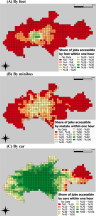
\includegraphics[width=1.33in]{images/4_access} 

}

\caption{\label{fig:access1} Oportunidades acessíveis em 60 minutos. Fonte: Nakamura e Avner (2021)}\label{fig:access, out.width:"35%"}
\end{figure}
\end{columns}
\end{frame}

\hypertarget{conclusuxe3o}{%
\subsection{Conclusão}\label{conclusuxe3o}}

\begin{frame}{Conclusão}
Dolor
\end{frame}

\hypertarget{obrigado}{%
\subsection{Obrigado!}\label{obrigado}}

\begin{frame}{Obrigado!}
Sit amet
\end{frame}

\end{document}
